\subsection{Wellenlängenselektion}

\subsubsection{Selektion über Reflektivität der Spiegel}

\paragraph{Aufbau und Durchführung}

Für diesen Versuchsteil wurde der in Abb.~\ref{img:aufbau4} beschriebene Aufbau verwendet mit dem
einzigen Unterschied, dass die Spiegel des Resonators gegen Spiegel mit hoher Transmission bei
445\,nm und hoher Reflektivität bei 525-610\,nm ausgetauscht wurden.
Durch Verändern der Ausrichtung des Kristalls ließ sich damit die grüne und gelbe Laserlinie
erzeugen. Es wurden jeweils die Ausgangsleistung sowohl bei 25\grad als auch bei 35\grad Pumplaser
Temperatur und Pumpströme zwischen 0\,A und 1.4\,A in 50\,mA Schritten gemessen.
Für die Leistungsmessung wurde der OP-2 VIS Powerhead (bis 30\,mW) verwendet.


\paragraph{Auswertung}
Die Abbildungen \ref{img:PI_gruen} und \ref{img:PI_gelb} zeigen die Kennlinien,
die so aufgenommen wurden.
Die Fehler wurden aus der Schwankung des Messwerts des Powerheads abgeschätzt.
Lineare Fits wurden wegen der starken Krümmung der Kennlinien nicht durchgeführt.

\begin{figure}[H]
\begin{center}
  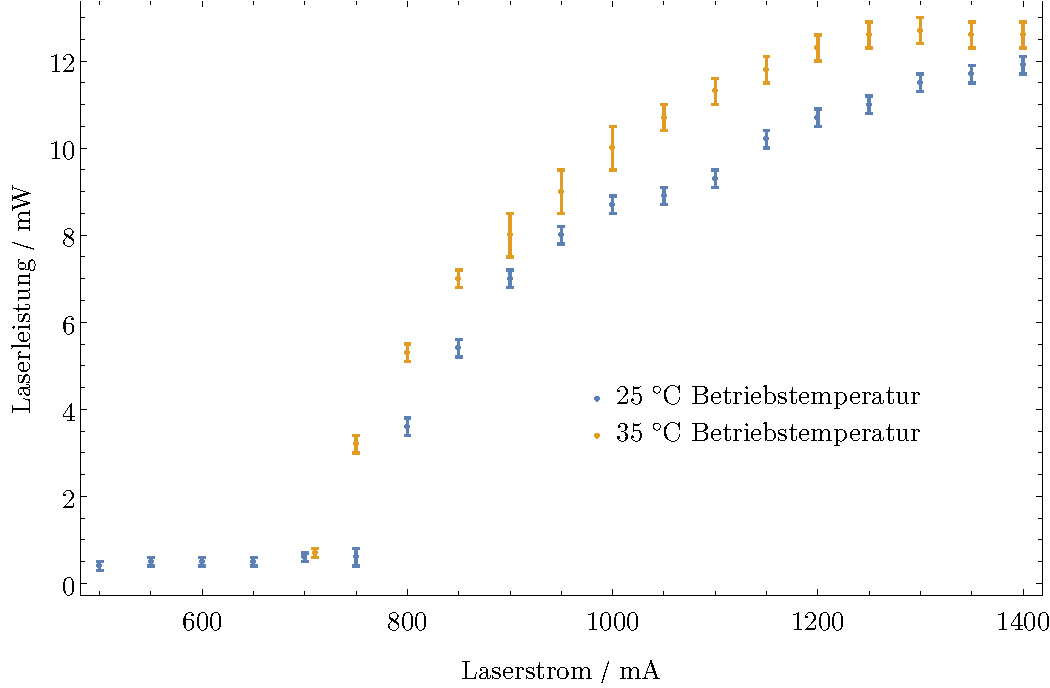
\includegraphics[width=.9\textwidth]{PI_gruen.pdf}
  \caption{PI-Kennlinie des grünen Lasers bei 25\grad und 35\grad
  Betriebstemperatur.}
  \label{img:PI_gruen}
\end{center}
\end{figure}


\begin{figure}[H]
\begin{center}
  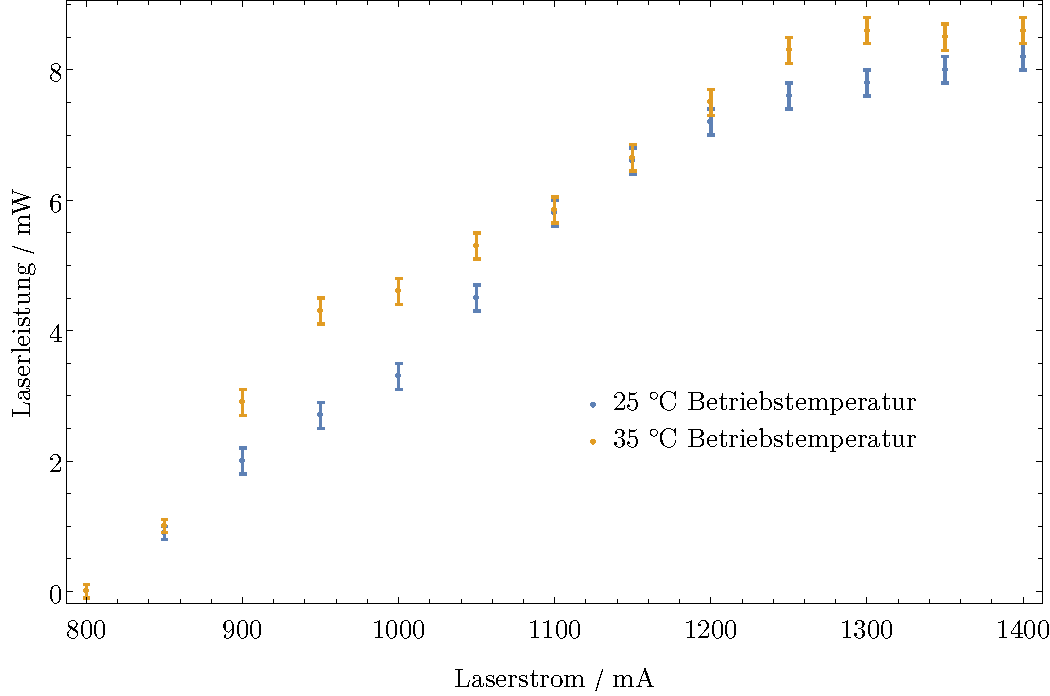
\includegraphics[width=.9\textwidth]{PI_gelb.pdf}
  \caption{PI-Kennlinie des gelben Lasers bei 25\grad und 35\grad
  Betriebstemperatur.}
  \label{img:PI_gelb}
\end{center}
\end{figure}



\subsubsection{Selektion über doppelbrechenden Kristall}


\paragraph{Aufbau und Durchführung}


\begin{figure}[H]
\begin{center}
  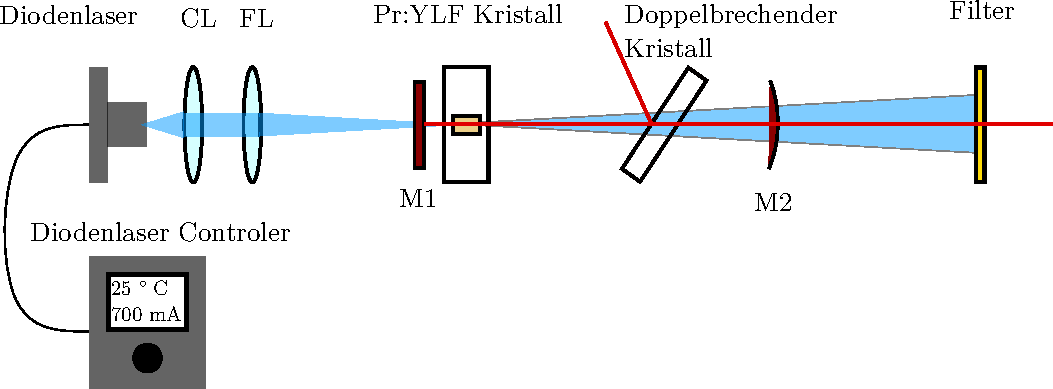
\includegraphics[width=\textwidth]{Aufbau5.pdf}
  \caption{Schematische Darstellung des Aufbaus zur Wellenlängenselektion mit doppelbrechendem Kristall.
   Der einzige Unterschied zu dem in Abb.~\ref{img:aufbau4} beschriebenem Aufbau ist der zusätzlich
  in dem Resonator untergebrachte doppelbrechende Kristall, welcher unter dem Brewsterwinkel von
  etwa 53$^\circ$ zur Strahlachse verkippt ist, um Reflexionsverluste zu minimieren.}
  \label{img:aufbau5}
\end{center}
\end{figure}

Der verwendete Aufbau ist in Abb.~\ref{img:aufbau5} dargestellt.
Für diesen Versuchsteil wurden wieder die Spiegel mit hoher Reflektivität bei 580-720\,nm verwendet.
Durch Rotieren des doppelbrechenden Kristalls sowie des Pr:YLF Kristalls konnte Lasing bei
verschiedenen Wellenlängen beobachtet werden. Der Strom des Pumplasers wurde dazu auf 1.4\,A
maximiert und die Temperatur auf 25\grad eingestellt. Der ausgekoppelte Strahl wurde auf einem
weißen Schirm betrachtet und dessen Spektrum über eine optische Faser mit dem Spektrometer
aufgenommen.



\paragraph{Auswertung}
Drei verschiedene Linien konnten so gefunden werden,
die Spektren sind auf Abb.~\ref{img:BifrSpekt} zu sehen:
Die gelbe Linie bei 607\,nm, die rote Linie bei 640\,nm und die dunkelrote Linie bei 721\,nm.



\begin{figure}[H]
\begin{center}
  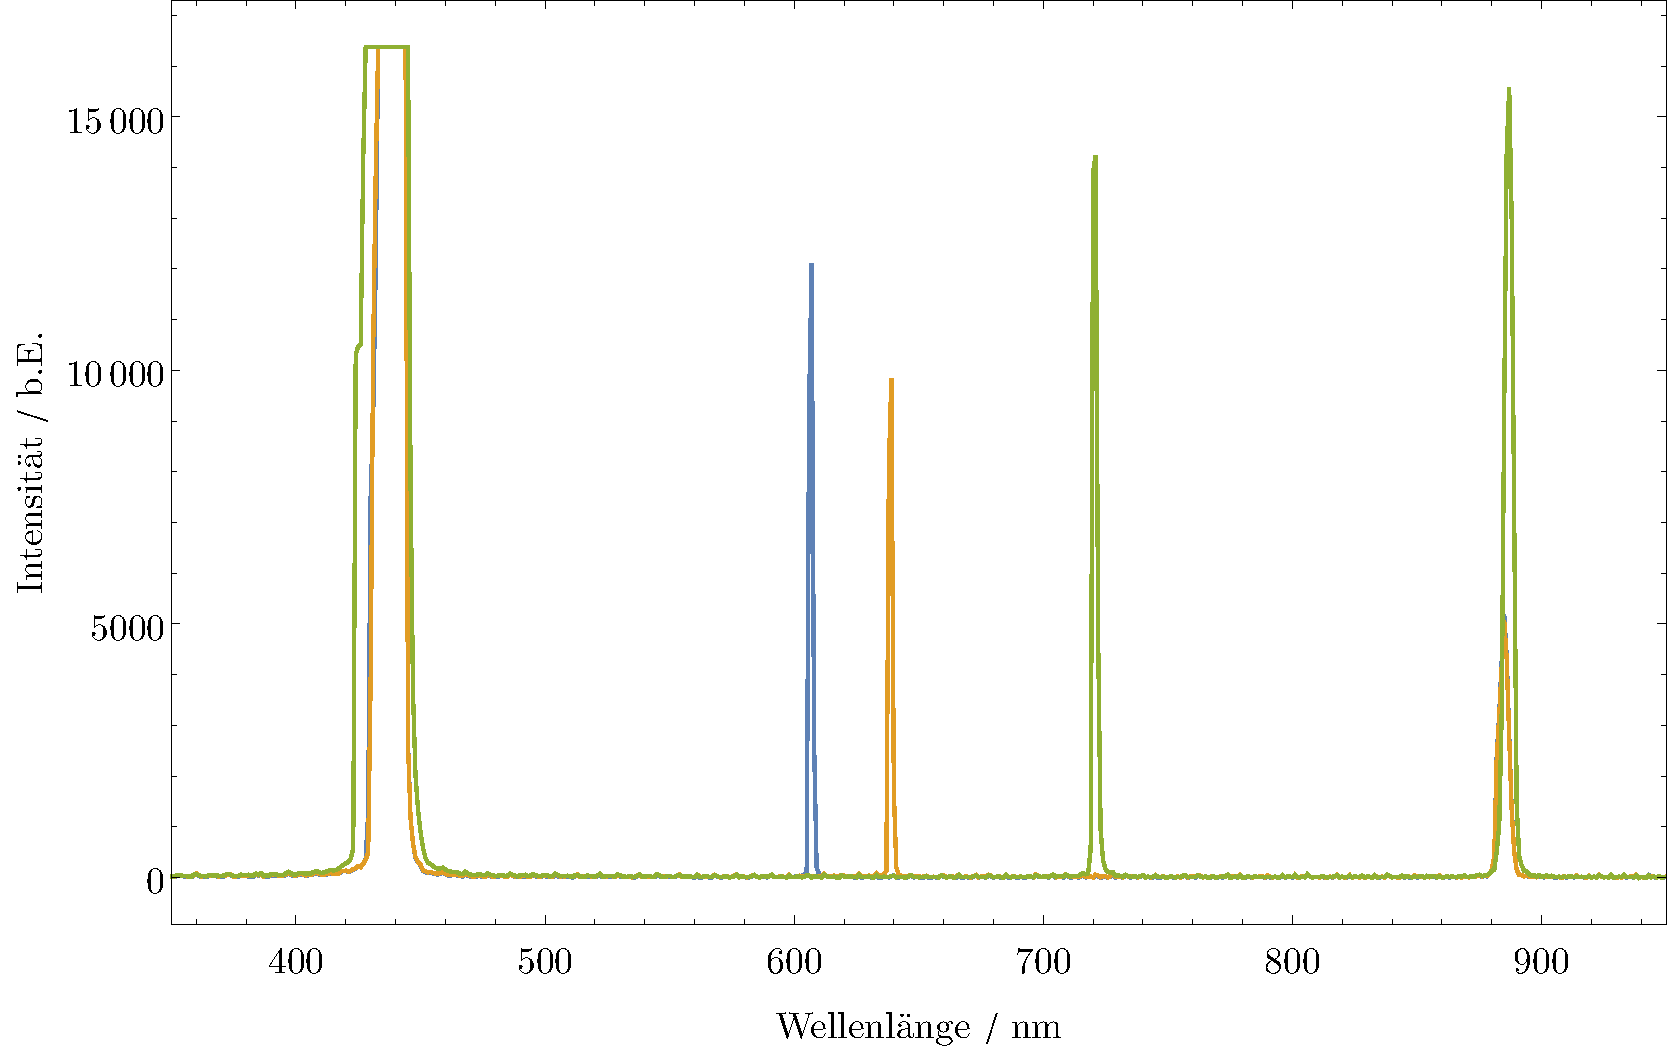
\includegraphics[width=.9\textwidth]{BifrSpekt.pdf}
  \caption{Spektren des Lasers für drei unterschiedliche Winkel des doppelbrechenden Kristalls.}
  \label{img:BifrSpekt}
\end{center}
\end{figure}

\subsubsection{Selektion mit Littrow-Prisma}

\paragraph{Aufbau und Durchführung}

\begin{figure}[H]
\begin{center}
  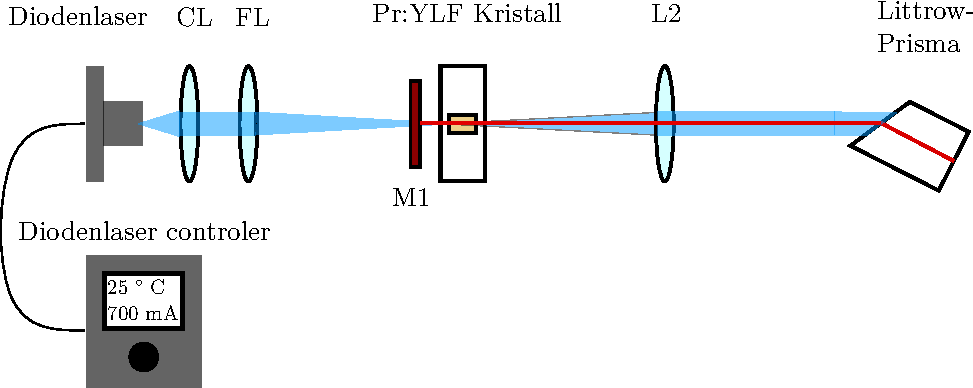
\includegraphics[width=.9\textwidth]{Aufbau6.pdf}
  \caption{Schematische Darstellung des Aufbaus zur Wellenlängenselektion mit einem Littrow-Prisma.
  Hinter den Kristall wird eine weitere Linse (L2) mit einer Brennweite von 50\,mm so
  platziert, dass ihr Brennpunkt im Inneren des Kristalls liegt und hinter ihr erneut ein
  kollimierter Strahl entsteht. Dahinter wird das Littrow-Prisma montiert, wobei der Abstand zum
  Kristall keine Rolle spielt.}
  \label{img:aufbau6}
\end{center}
\end{figure}

Abb.~\ref{img:aufbau6} zeigt den zur Wellenlängenselektion mit einem Littrow-Prisma verwendeten
Aufbau. Durch Verkippen des Prismas und gleichzeitigem Rotieren des Kristalls konnte Lasing bei
verschiedenen Wellenlängen eingestellt werden. Das Spektrum wurde erneut mithilfe einer optischen
Faser, die auf das Littrow-Prisma gerichtet wurde, über das Spektrometer aufgenommen.
Außerdem wurden grob die Winkelbereiche des Pr:YLF-Kristalls notiert, bei dem Lasing
mit den verschiedenen Wellenlängen auftrat.
Der Pumplaser wurde wieder bei 1.4\,A und 25\grad betrieben.

\paragraph{Auswertung}
Die gefundenen drei Linien (Abb.~\ref{img:LittrSpekt}) sind die gleichen wie bei der Messung mit dem
doppelbrechenden Kristall.
Für die rote Linie bei 640\,nm wurde folgende Abhängigkeit von der Rotation des Pr:YLF-Kristalls
festgestellt:
Bei einer vollständigen Rotation um 360$^\circ$ treten zwei Maxima der Intensität auf, die sich
gegenüberliegen.
Lasing ist bei Drehungen um bis zu $\pm\,45^\circ$ aus dem Intensitätsmaximum möglich.

Die dunkelrote Linie besitzt die gleiche Winkelabhängigkeit,
sie ist allerdings um 90$^\circ$ verschoben: Bei den Maxima der hellroten Linie besitzt die
dunkelrote Linie Minima.


\begin{figure}[H]
\begin{center}
  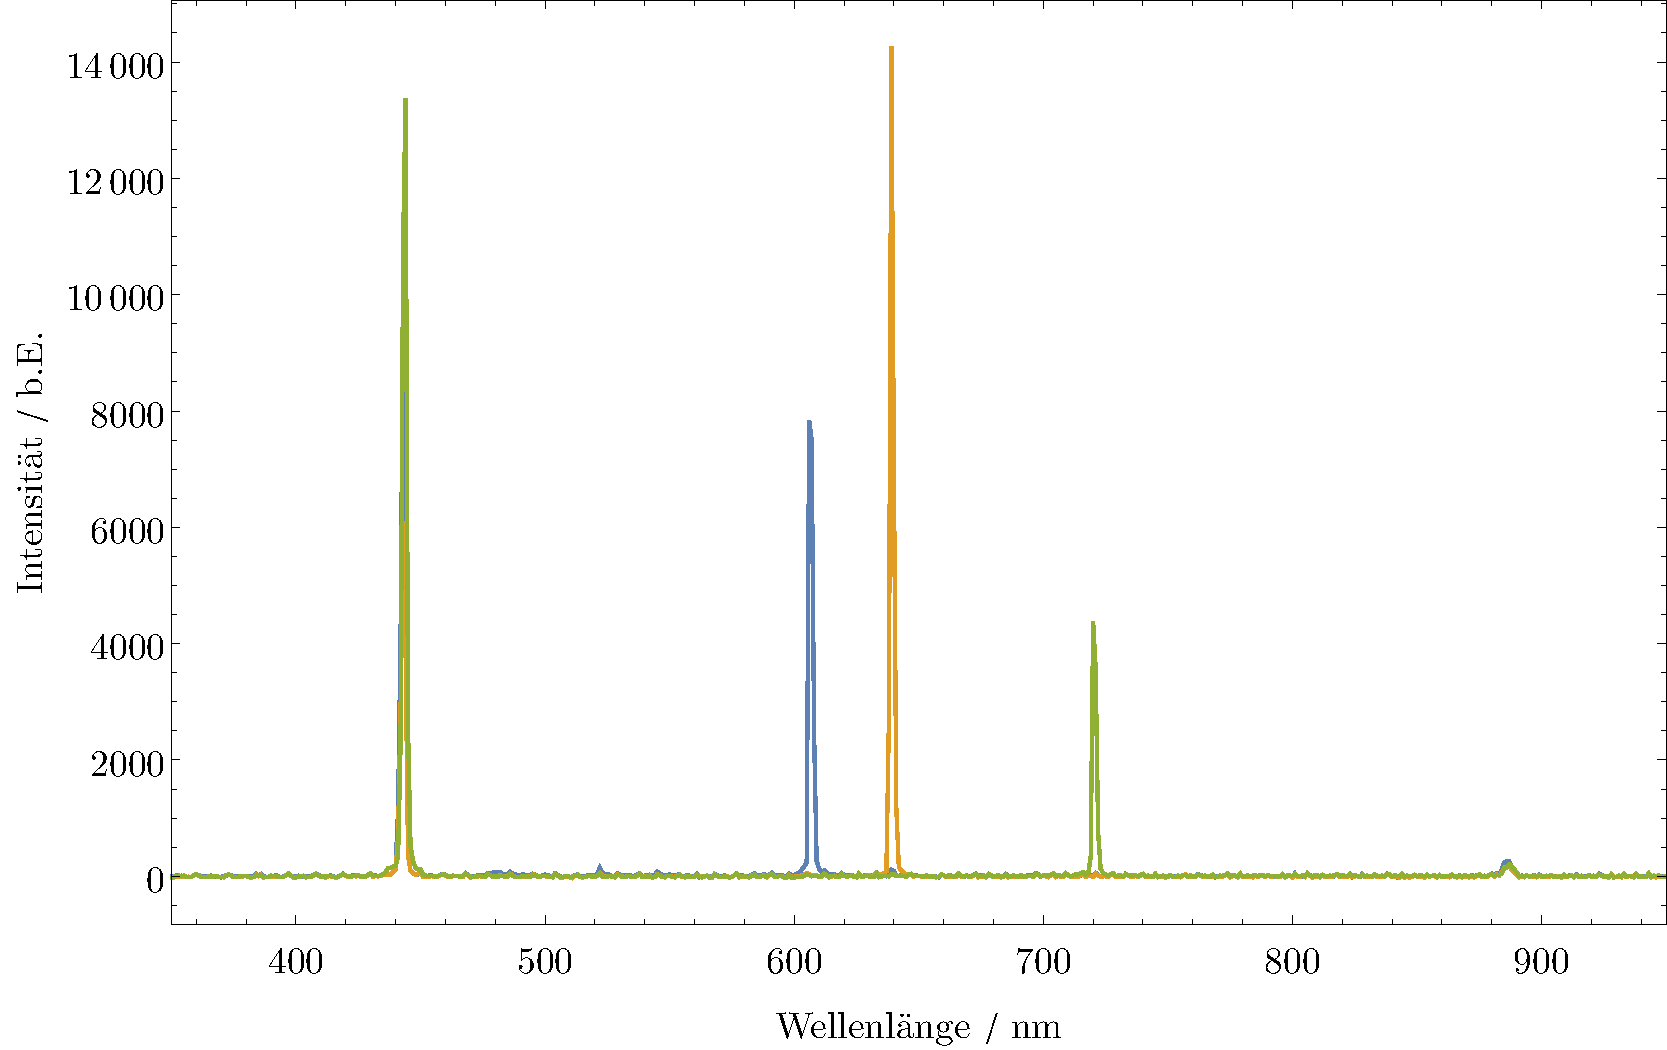
\includegraphics[width=\textwidth]{LittrSpekt.pdf}
  \caption{Spektren des Lasers für drei unterschiedliche Einstellungen des Littrow-Prismas.}
  \label{img:LittrSpekt}
\end{center}
\end{figure}
